
\subsection{Skyline Computation}

Techniques of computation of skyline records in traditional
database systems have been studied in \cite{skyline_operator},
\cite{shooting_stars}, and \cite{progressive_skyline}. The well
known algorithms are Nest-Loop, Block-Nested-Loop, and Divide and
Conquer. The Nest-Loop algorithm is an intuitive way to compute
skyline points in the way that every record is compared with every
other records in a table to determine if the record is dominated.
In Block-Nested-Loop, a record is only compared with other records
in the same block. The candidate skyline points in each block is
compare to obtain the final skyline points. In Divide and Conquer
(D\&C), the data set is recursively divided until there are only
two records. Skyline points are calculated for each segment
produced in the division phase. The division phase is followed by
a merge phase in which the skyline of all divisions are compare
and merge to obtain the final skyline set.

\cite{shooting_stars} introduces an online skyline computation
algorithm in which the skyline are computed progressively. The
first skyline is return almost immediately and more skyline points
are added to the result set.

Nearest Neighbor (NN) and Branch-and-Bound (BBS) skyline
algorithms are two of the best performing algorithms for
progressive skyline computation for traditional database systems
presented in \cite{progressive_skyline}. In NN skyline algorithm,
the records of the data set are presented geometrically in a
Euclidean space with the relevant attributes as the coordinate in
each dimension. In the example of hotel close to the ocean in
previously presented, a record would be placed on a plane with the
distance of the hotel to the ocean and its price as the two axis
that determine and the values in the two attributes as the
coordinates of the records on the Euclidean plane as in Figure
\ref{fig:skyline_nn}. The NN algorithm finds a nearest neighbor
from the axes and that is the first skyline point. Then the
algorithm marks the region that is dominated by the first skyline
point so that anything in that region will not be searched. The
search results in two more search regions and the search continues
until no more records are left.

\begin{figure}[h]
\begin{center}
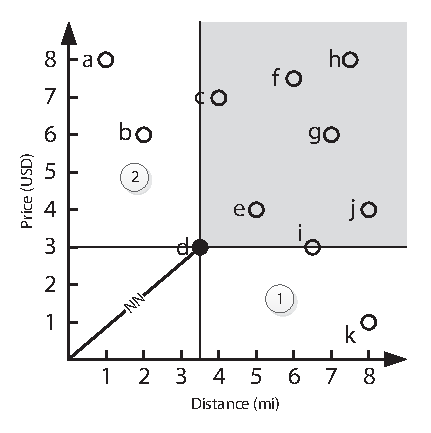
\includegraphics[width=2in]{Figures/skyline_nn.eps}
\caption{\small NN d and its pruning region.
\label{fig:skyline_nn}}
\end{center}
\end{figure}

BBS is an algorithm that surpass the computation efficiency of the
NN algorithm. BBS utilizes the best first search technique to
traverse the index tree to prune the branches unnecessary
branches. Unfortunately, both NN and BBS can not be easily adopted
to the broadcast environment due to the linear nature of broadcast
program. Both NN and BBS requires backtracking of the index tree
to find the best path to prune, which is impermissible in
broadcast environment or require waiting for the next broadcast
cycle, which incurs long waiting time. The solutions presented in
this paper will use the pruning regions strategy used in NN. Our
algorithms systematically builds pruning regions, as presented in
NN algorithm, as the client receives and discovers more data from
the broadcast channel.


\subsection{Wireless Broadcast Index}\label{sec:wireless_bcast_index}
Many excellent studies have been done on improving efficiency of
wireless broadcast system using indexing techniques. This section
considers several popular index allocation techniques and
discusses benefits and drawbacks.

The intuitive technique of no index and one-time index at
beginning of a broadcast cycle has been considered in
\cite{data_on_air}. With no index, the length of a cycle is
minimized, but the tuning time is the entire cycle since the
program is not self-descriptive. With one-time index, the clients
are able to filter unwanted data and reduce tuning time, but if a
client misses the one-time index, then it will have to wait until
the next cycle even if there is useful data in current cycle.

$(1, m)$ indexing, proposed by Imielinski, et al. in
\cite{data_on_air}, is a mitigation to the problem of one-time
index by replicating the entire index every $1/m$ length of the
broadcast cycle. The benefit of this index technique is when a
client misses an index segment, it can wait for the next index in
the same cycle \cite{DBLP:journals/tmc/KuZW08}. The drawback of
this technique is the space consumption of replicating the full
index several times in the cycle.

Distributed index was also proposed in \cite{data_on_air}. This
index also replicate the index in the broadcast cycle, but only a
part of the index is replicated. Advantages of this method are (1)
index can be obtained throughout cycle, (2) reduced bandwidth
consumption comparing with $(1, m)$, and (3) not limited to
particular index structure.

%\cite{data_on_air} by Imielinski, et al. is an
%early and influential work of data
%indexing for broadcast on air. The paper defined two
%characteristics of wireless broadcast, \em{tuning time} and \em{access latency}. Tuning time
%defines how long the client has to actively listen on the channel to get all the desired data.
%Access latency define the time when the client issues the query to the time all the desired
%data is received. Tuning time is proportional to power usage of mobile clients. The goal is to
%reduce both tuning time and access latency.

%In addition, the paper also proposed a few air index techniques to reduce client tuning time.
%The first index proposed is $(1, m)$ index, in which the full index is repeated every $1/m$ of
%the entire broadcast cycle. The index is repeat so that clients that tune into the channel in
%the middle of the broadcast does not have to wait until the next cycle to get the index and
%process request. The second index proposed is the distributed index, in which only a part of
%the index is repeated. Distributed index reduces the overhead of embedding index and improves
%access latency.

Data filtering based on data signature was proposed in
\cite{signature_and_caching}. During data retrieval, the signature
of desire data is compared with the signature of a data segment
prepared by the broadcast server. If the signatures match, then
data is downloaded, else ignored.

Distributed index for spatial data in error-prone air broadcast
was introduced in \cite{dsi}. Instead of replication, his paper
proposes a distributed index in the broadcast cycle with no
duplicate of index. The paper index broadcast spatial data using
Hilbert values. Each data record contains an index table that
contains the data segments that will be pushed onto the channel in
the near future. A drawback of this approach is the lose of
spatial precision due to the use of space filling curve as index.


%\section{System Model}

%In our theoretical model, the system consists of the broadcast server and multiple clients. As
%discussed in section 2.1, the server periodically broadcast data in a specific channel. Any client
%that is interested in any of the data serviced by the server tunes into the channel to get the
%desire data. The server contains a set of records as illustrated in Figure 4.

%In this model, we assume a pure broadcast model in which all data are transmitted through downlink
%bandwidth and that there is not uplink bandwidth. Clients must tune into the channel as long as it
%takes to obtain all desire data. Apparently, in order to support efficient query, the server must
%provide data index so that the client can tune in only when the relevant data is to be broadcasted
%In addition, this model contains only one transmission channel. Index must be transmitted on the
%same channel as the data.
